\documentclass[]{article}
\usepackage{amssymb,amsmath}
\usepackage{ifxetex,ifluatex}
\ifxetex
  \usepackage{fontspec,xltxtra,xunicode}
  \defaultfontfeatures{Mapping=tex-text,Scale=MatchLowercase}
\else
  \ifluatex
    \usepackage{fontspec}
    \defaultfontfeatures{Mapping=tex-text,Scale=MatchLowercase}
  \else
    \usepackage[utf8]{inputenc}
  \fi
\fi
\usepackage{ctable}
\usepackage{float} % provides the H option for float placement
\usepackage{graphicx}
% We will generate all images so they have a width \maxwidth. This means
% that they will get their normal width if they fit onto the page, but
% are scaled down if they would overflow the margins.
\makeatletter
\def\maxwidth{\ifdim\Gin@nat@width>\linewidth\linewidth
\else\Gin@nat@width\fi}
\makeatother
\let\Oldincludegraphics\includegraphics
\renewcommand{\includegraphics}[1]{\Oldincludegraphics[width=\maxwidth]{#1}}
\ifxetex
  \usepackage[setpagesize=false, % page size defined by xetex
              unicode=false, % unicode breaks when used with xetex
              xetex,
              colorlinks=true,
              linkcolor=blue]{hyperref}
\else
  \usepackage[unicode=true,
              colorlinks=true,
              linkcolor=blue]{hyperref}
\fi
\hypersetup{breaklinks=true, pdfborder={0 0 0}}
\setlength{\parindent}{0pt}
\setlength{\parskip}{6pt plus 2pt minus 1pt}
\setlength{\emergencystretch}{3em}  % prevent overfull lines
\setcounter{secnumdepth}{0}

\title{Outlier tests}
\author{Rapport package team @ https://github.com/aL3xa/rapport}
\date{2011-04-26 20:25 CET}

\begin{document}
\maketitle

\subsection{Description}

This template will check if provided variable has any outliers.

\subsection{Boxplot}

\href{ea1797865a9d9a619be0e9c5d55d5de7-hires.png}{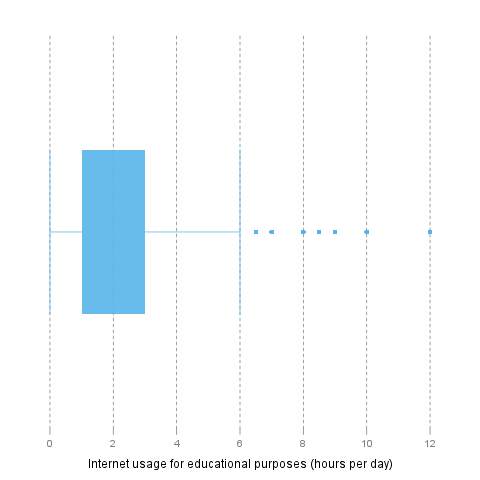
\includegraphics{ea1797865a9d9a619be0e9c5d55d5de7.png}}

\subsection{Lund test}

It seems that \emph{4} extreme values can be found in ``Internet usage
for educational purposes (hours per day)''. These are: 10, 0.5, 1.5,
0.5.

\subsubsection{Explanation}

The above test for outliers was based on \emph{lm(1 \ensuremath{\sim}
edu)}:

\ctable[pos = H, center, botcap]{lllll}
{% notes
}
{% rows
\FL
 & \textbf{Estimate} & \textbf{Std. Error} & \textbf{t
value} & \textbf{Pr(\textgreater{}\textbar{}t\textbar{})}
\ML
(Intercept) & 2.0481 & 0.078 & 26.2677 & 0
\LL
}

\subsubsection{References}

\begin{itemize}
\item
  Lund, R. E. 1975, ``Tables for An Approximate Test for Outliers in
  Linear Models'', Technometrics, vol.~17, no. 4, pp.~473-476.
\item
  Prescott, P. 1975, ``An Approximate Test for Outliers in Linear
  Models'', Technometrics, vol.~17, no. 1, pp.~129-132.
\end{itemize}
\subsection{Grubb's test}

Grubbs test for one outlier shows that highest value 12 is an outlier
(p=0.0002).

\subsubsection{References}

\begin{itemize}
\item
  Grubbs, F.E. (1950). Sample Criteria for testing outlying
  observations. Ann. Math. Stat. 21, 1, 27-58.
\end{itemize}
\subsection{Dixon's test}

chi-squared test for outlier shows that highest value 12 is an outlier
(p=0).

\subsubsection{References}

\begin{itemize}
\item
  Dixon, W.J. (1950). Analysis of extreme values. Ann. Math. Stat. 21,
  4, 488-506.
\end{itemize}
\subsection{Description}

This template will check if provided variable has any outliers.

\subsection{Boxplot}

\href{ea1797865a9d9a619be0e9c5d55d5de7-hires.png}{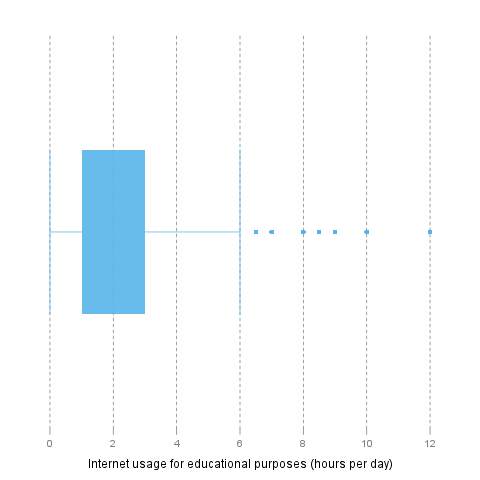
\includegraphics{ea1797865a9d9a619be0e9c5d55d5de7.png}}

\subsection{Lund test}

It seems that \emph{4} extreme values can be found in ``Internet usage
for educational purposes (hours per day)''. These are: 10, 0.5, 1.5,
0.5.

\subsubsection{Explanation}

The above test for outliers was based on \emph{lm(1 \ensuremath{\sim}
edu)}:

\ctable[pos = H, center, botcap]{lllll}
{% notes
}
{% rows
\FL
 & \textbf{Estimate} & \textbf{Std. Error} & \textbf{t
value} & \textbf{Pr(\textgreater{}\textbar{}t\textbar{})}
\ML
(Intercept) & 2.0481 & 0.078 & 26.2677 & 0
\LL
}

\subsubsection{References}

\begin{itemize}
\item
  Lund, R. E. 1975, ``Tables for An Approximate Test for Outliers in
  Linear Models'', Technometrics, vol.~17, no. 4, pp.~473-476.
\item
  Prescott, P. 1975, ``An Approximate Test for Outliers in Linear
  Models'', Technometrics, vol.~17, no. 1, pp.~129-132.
\end{itemize}
\subsection{Grubb's test}

Grubbs test for one outlier shows that highest value 12 is an outlier
(p=0.0002).

\subsubsection{References}

\begin{itemize}
\item
  Grubbs, F.E. (1950). Sample Criteria for testing outlying
  observations. Ann. Math. Stat. 21, 1, 27-58.
\end{itemize}
\subsection{Dixon's test}

chi-squared test for outlier shows that highest value 12 is an outlier
(p=0).

\subsubsection{References}

\begin{itemize}
\item
  Dixon, W.J. (1950). Analysis of extreme values. Ann. Math. Stat. 21,
  4, 488-506.
\end{itemize}
\subsection{Description}

This template will check if provided variable has any outliers.

\subsection{Boxplot}

\href{ea1797865a9d9a619be0e9c5d55d5de7-hires.png}{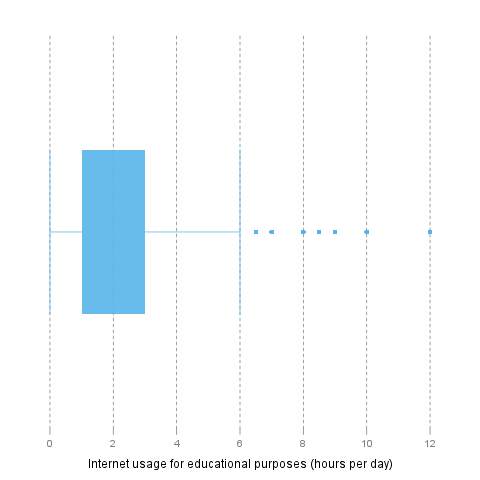
\includegraphics{ea1797865a9d9a619be0e9c5d55d5de7.png}}

\subsection{Lund test}

It seems that \emph{4} extreme values can be found in ``Internet usage
for educational purposes (hours per day)''. These are: 10, 0.5, 1.5,
0.5.

\subsubsection{Explanation}

The above test for outliers was based on \emph{lm(1 \ensuremath{\sim}
edu)}:

\ctable[pos = H, center, botcap]{lllll}
{% notes
}
{% rows
\FL
 & \textbf{Estimate} & \textbf{Std. Error} & \textbf{t
value} & \textbf{Pr(\textgreater{}\textbar{}t\textbar{})}
\ML
(Intercept) & 2.0481 & 0.078 & 26.2677 & 0
\LL
}

\begin{center}\rule{3in}{0.4pt}\end{center}

This report was generated with \href{http://www.r-project.org/}{R}
(2.14.0) and \href{http://al3xa.github.com/rapport/}{rapport} (0.1) in
1.157 sec on x86\_64-unknown-linux-gnu platform.

\begin{figure}[htbp]
\centering

\includegraphics{images/logo.png}
\caption{}
\end{figure}

\end{document}
